\documentclass[12pt]{report}                  % Times New Roman, 12pt
%\usepackage{gscale_thesis_singlespace} % Single spaced thesis
\usepackage{gscale_thesis_doublespace} % Double spaced thesis
\usepackage{fancyheadings}                   % Header and footer styling
\usepackage{natbib}                               % Bibliography formatting
\usepackage{setspace}                           % Allows double spacing but skips headers/footers
\title{1000 Plagues in the Genomics Age}
\halftitle{Plague Genomics} % 60 Characters Max. Including Spaces

\author{Katherine Eaton}
\shortauthor{K. Eaton} % Used for page header

\dept{Department of Anthropology} % The department you are part of; Must be all lower case
\field{Ancient DNA} % What field your thesis is in

\degree{Doctor of Philosophy}
\prevdegreeone{B.A. (Hons) Anthropology,\\ University of Alberta, Edmonton, Canada}
\prevdegreetwo{B.A. (Hons)}

\submitdate{June 2021}
\copyrightyear{2021}

\principaladviser{Dr. Hendrik Poinar} % Your Supervisor
                                % LaTeX variables for preface pages/headers
\setcounter{tocdepth}{1}                        % Limits the TOC to chapter and section names

% Additional packages
\usepackage{graphicx}                                   % Allows the inclusion of figures
\usepackage{subcaption}                               % Allows captions to be added to subfigures
\usepackage[justification=centering]{caption} % Centres caption text
\usepackage[hidelinks]{hyperref}                    % Linking to LaTeX labels and external URLs
\usepackage{array}                                        % Used for table formatting
\newcolumntype{P}[1]{>{\raggedright\let\newline\\\arraybackslash\hspace{0pt}}m{#1}}
\usepackage{booktabs}                                 % Fancy-style tables
\usepackage{longtable}                                 % Allows for tables that are more than one page long
\usepackage{float}                                         % Better figure placement control
\usepackage{enumerate}   
\usepackage[shortlabels]{enumitem}                            % Numbered lists 
\usepackage[shortcuts]{extdash}                  % Allows manual hyphenation of hypenated words
\usepackage{amsmath}                                % Non-standard math symbols
\usepackage{amsfonts}                                % Extended fonts for mathematics
\usepackage{xcolor}
\numberwithin{equation}{section}                 % Numbers equations based on their section

% ********************************
\begin{document}
\beforepreface                                         % Half title page, title page, declaration page   
  \prefacesection{Lay Abstract}

A lay abstract of not more 150 words must be included explaining the key goals and contributions of the thesis in lay terms that is accessible to the general public.                                   % Lay Abstract
  \prefacesection{Abstract}

Abstract here (no more than 300 words)                                      % Abstract
  %\thispagestyle{empty}
\null\vfill
\begin{center}
%\textbf{Dedications}
%\linebreak
\textsl{Your Dedication \\ Optional second line}
\end{center}
\vfill
                                      % Dedication
  \prefacesection{Acknowledgements}

Acknowledgements go here.                 % Acknowledgements
  \referencepageswithnotations{notation} % Table of Contents, List of Figures, List of Tables, Notations
  %\referencepages                                 % No notations version (choose one)
\afterpreface                      
  
  
  \chapter{Introduction}

Every thesis needs an introductory chapter                  
        \setcounter{figure}{0}
        \setcounter{equation}{0}
        \setcounter{table}{0}
        
  \chapter{Your Chapter Title}

This is a sample chapter

\section{Referencing}
These are some sample references to GAMYGDALA~\citep{popescu2014gamygdala} from the ``refernces.bib" file and state effects of cognition~\citep{hudlicka2002time} from the ``reference\_another.bib" file. These references are not in the same .bib file.

\section{Figures}
This is a single image figure (Figure~\ref{fig_singleenv}:

\begin{figure}[ht]
	\centering
	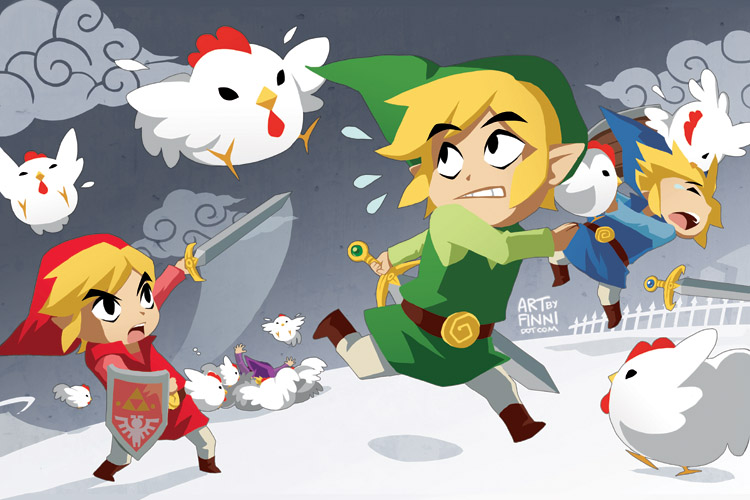
\includegraphics[width=0.6\textwidth]{figures/Sample/tumblr_static_eaceks0rfxsss8o4swscw40wo.jpg}
	\caption[Single Figure Environment Listed Title]{This is a single figure environment}
	\label{fig_singleenv}
\end{figure}

This is a multi-image figure with a top (Figure~\ref{fig_multienv_1}) and bottom (Figure~\ref{fig_multienv_2}) aligned subfigures:

\begin{figure}[ht]
	\centering
	\begin{subfigure}[t]{\textwidth}
		\centering
		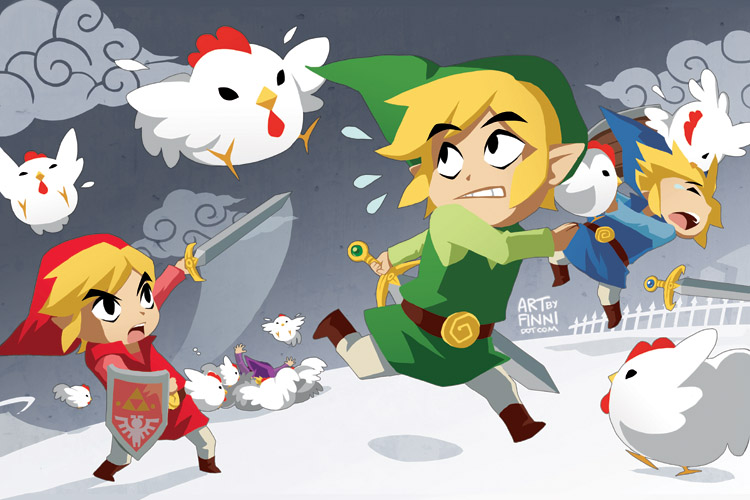
\includegraphics[width=0.7\textwidth]{figures/Sample/tumblr_static_eaceks0rfxsss8o4swscw40wo.jpg}
		\caption{Figure 1}
		\label{fig_multienv_1}
	\end{subfigure}
	~
	\begin{subfigure}[t]{\textwidth}
		\centering
		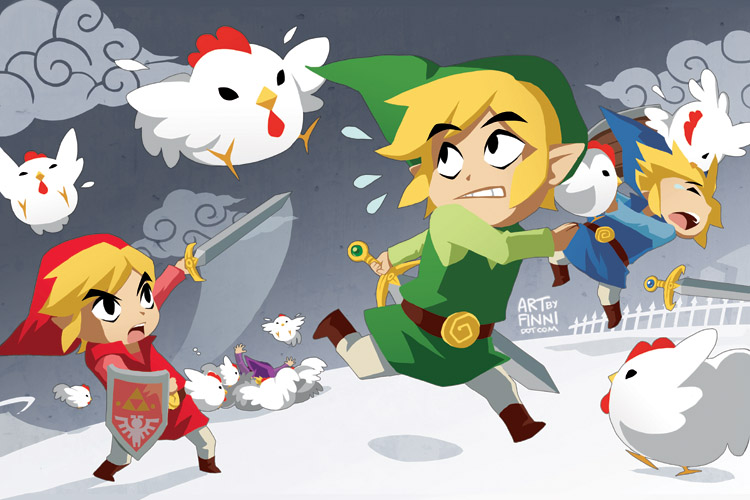
\includegraphics[width=0.7\textwidth]{figures/Sample/tumblr_static_eaceks0rfxsss8o4swscw40wo.jpg}
		\caption{Figure 2}
		\label{fig_multienv_2}
	\end{subfigure}
	
	\caption{A Multi-Figure Environment}
	\label{fig_multienv}
\end{figure}

\section{Tables}

Here is a sample table (Table~\ref{tab_sample}):

	\begin{table}[ht]
	\centering
	\begin{tabular}{ m{0.2\textwidth} m {0.1\textwidth} m{0.15\textwidth} }
		\toprule
		A & $\longleftrightarrow$ & B \\
		C & $\longleftrightarrow$ & D \\
		\bottomrule	
	\end{tabular}	
	\caption{A sample table}	
	\label{tab_sample}
\end{table}

\subsection{Long Tables}
A sample long table is shown in Appendix~\ref{appendix_b}.

\section{Equations}

Here is a sample equation (Equation~\ref{eq_lineslope}):

\begin{equation} \label{eq_lineslope}
	y = mx + b
\end{equation}                  
       \setcounter{figure}{0}
       \setcounter{equation}{0}
       \setcounter{table}{0}

  \chapter{Conclusion}

Every thesis also needs a concluding chapter
        \setcounter{figure}{0}
        \setcounter{equation}{0}
        \setcounter{table}{0}

\begin{appendix}
	\chapter{Your Appendix}
\label{appendix_a}

Your appendix goes here.

		\setcounter{figure}{0}
		\setcounter{equation}{0}
		\setcounter{table}{0}
		
	\chapter{Long Tables}
\label{appendix_b}

This appendix demonstrates the use of a long table that spans multiple pages.

\begin{center}
\begin{longtable}{P{3cm}P{3cm}P{2.5cm}P{3.5cm}}
\toprule
\hline
\textbf{Col A} & \textbf{Col B} & \textbf{Col C} & \textbf{Col D} \\ \midrule

\endfirsthead
\multicolumn{4}{c}{\textit{Continued from previous page}} \\ \hline
\textbf{Col A} & \textbf{Col B} & \textbf{Col C} & \textbf{Col D} \\ \hline
\endhead
\hline \multicolumn{4}{r}{\textit{Continued on the next page}} \\
\endfoot
\hline
\endlastfoot

A & B & C & D \\ \midrule

A & B & C & D \\ \midrule

A & B & C & D \\ \midrule

A & B & C & D \\ \midrule

A & B & C & D \\ \midrule

A & B & C & D \\ \midrule

A & B & C & D \\ \midrule

A & B & C & D \\ \midrule

A & B & C & D \\ \midrule

A & B & C & D \\ \midrule

A & B & C & D \\ \midrule

A & B & C & D \\ \midrule

A & B & C & D \\ \midrule

A & B & C & D \\ \midrule

A & B & C & D \\ \midrule

A & B & C & D \\ \midrule

A & B & C & D \\ \midrule

A & B & C & D \\ \midrule

A & B & C & D \\ \midrule

A & B & C & D \\ \midrule

\hline
\end{longtable}
\end{center}

		\setcounter{figure}{0}
		\setcounter{equation}{0}
		\setcounter{table}{0}
\end{appendix}

% The bibliography is set up to allow for multiple bib files
\bibliographystyle{natbib}
\bibliography{references,references_another}

\label{NumDocumentPages}

\end{document}
% ********************************
